% Author: Xu Chen, University of Washington
% Lab 02 homework scene: the SUV. Only what homework.md gives (no hidden model or grade values).
\documentclass[border=4pt]{standalone}
% Author: Xu Chen, University of Washington
% Shared TikZ style for the Control in Practice scene figures. % Author: Xu Chen, University of Washington
% Shared TikZ style for the Control in Practice scene figures. % Author: Xu Chen, University of Washington
% Shared TikZ style for the Control in Practice scene figures. \input{../../../docs/figures/cipstyle} from a lab.
\usepackage{amsmath,amssymb}
\usepackage[T1]{fontenc}
\usepackage{lmodern}
\usepackage{tikz}
\usepackage[siunitx]{circuitikz}
\usetikzlibrary{arrows.meta,calc,positioning,decorations.pathmorphing,decorations.markings,patterns,shapes.geometric,shadings,fit,backgrounds}
% restrained palette
\definecolor{ink}{HTML}{1A1A1A}
\definecolor{steel}{HTML}{8C96A0}
\definecolor{metal}{HTML}{D5DAE0}
\definecolor{accent}{HTML}{1F4E79}   % controller, signals we choose
\definecolor{plantc}{HTML}{FBE7D6}   % plant fill
\definecolor{sensorc}{HTML}{DCE8F3}  % sensor fill
\definecolor{dist}{HTML}{B03A2E}     % disturbances, forces from the environment
\definecolor{act}{HTML}{2E7D4F}      % actuation
\definecolor{note}{HTML}{555555}
\tikzset{
  every picture/.style={line width=0.8pt, >={Stealth[length=2.4mm]}, font=\small},
  thin line/.style={line width=0.5pt},
  thick line/.style={line width=1.2pt},
  dim/.style={thin line, note, {Stealth[length=1.6mm]}-{Stealth[length=1.6mm]}},
  ground/.style={pattern=north east lines, pattern color=steel, draw=none},
  block/.style={draw=ink, rounded corners=1.5pt, minimum height=9mm, minimum width=16mm, align=center, fill=white},
  plant/.style={block, fill=plantc},
  sensor/.style={block, fill=sensorc},
  ctrl/.style={block, draw=accent, text=accent, thick line},
  sum/.style={draw=ink, circle, minimum size=5mm, inner sep=0pt},
  sig/.style={->, ink},
  distsig/.style={->, dist, thick line},
  force/.style={-{Stealth[length=3mm]}, thick line},
  panel title/.style={font=\normalsize\bfseries, anchor=west, ink},
  caption/.style={font=\footnotesize, note, align=left},
}
 from a lab.
\usepackage{amsmath,amssymb}
\usepackage[T1]{fontenc}
\usepackage{lmodern}
\usepackage{tikz}
\usepackage[siunitx]{circuitikz}
\usetikzlibrary{arrows.meta,calc,positioning,decorations.pathmorphing,decorations.markings,patterns,shapes.geometric,shadings,fit,backgrounds}
% restrained palette
\definecolor{ink}{HTML}{1A1A1A}
\definecolor{steel}{HTML}{8C96A0}
\definecolor{metal}{HTML}{D5DAE0}
\definecolor{accent}{HTML}{1F4E79}   % controller, signals we choose
\definecolor{plantc}{HTML}{FBE7D6}   % plant fill
\definecolor{sensorc}{HTML}{DCE8F3}  % sensor fill
\definecolor{dist}{HTML}{B03A2E}     % disturbances, forces from the environment
\definecolor{act}{HTML}{2E7D4F}      % actuation
\definecolor{note}{HTML}{555555}
\tikzset{
  every picture/.style={line width=0.8pt, >={Stealth[length=2.4mm]}, font=\small},
  thin line/.style={line width=0.5pt},
  thick line/.style={line width=1.2pt},
  dim/.style={thin line, note, {Stealth[length=1.6mm]}-{Stealth[length=1.6mm]}},
  ground/.style={pattern=north east lines, pattern color=steel, draw=none},
  block/.style={draw=ink, rounded corners=1.5pt, minimum height=9mm, minimum width=16mm, align=center, fill=white},
  plant/.style={block, fill=plantc},
  sensor/.style={block, fill=sensorc},
  ctrl/.style={block, draw=accent, text=accent, thick line},
  sum/.style={draw=ink, circle, minimum size=5mm, inner sep=0pt},
  sig/.style={->, ink},
  distsig/.style={->, dist, thick line},
  force/.style={-{Stealth[length=3mm]}, thick line},
  panel title/.style={font=\normalsize\bfseries, anchor=west, ink},
  caption/.style={font=\footnotesize, note, align=left},
}
 from a lab.
\usepackage{amsmath,amssymb}
\usepackage[T1]{fontenc}
\usepackage{lmodern}
\usepackage{tikz}
\usepackage[siunitx]{circuitikz}
\usetikzlibrary{arrows.meta,calc,positioning,decorations.pathmorphing,decorations.markings,patterns,shapes.geometric,shadings,fit,backgrounds}
% restrained palette
\definecolor{ink}{HTML}{1A1A1A}
\definecolor{steel}{HTML}{8C96A0}
\definecolor{metal}{HTML}{D5DAE0}
\definecolor{accent}{HTML}{1F4E79}   % controller, signals we choose
\definecolor{plantc}{HTML}{FBE7D6}   % plant fill
\definecolor{sensorc}{HTML}{DCE8F3}  % sensor fill
\definecolor{dist}{HTML}{B03A2E}     % disturbances, forces from the environment
\definecolor{act}{HTML}{2E7D4F}      % actuation
\definecolor{note}{HTML}{555555}
\tikzset{
  every picture/.style={line width=0.8pt, >={Stealth[length=2.4mm]}, font=\small},
  thin line/.style={line width=0.5pt},
  thick line/.style={line width=1.2pt},
  dim/.style={thin line, note, {Stealth[length=1.6mm]}-{Stealth[length=1.6mm]}},
  ground/.style={pattern=north east lines, pattern color=steel, draw=none},
  block/.style={draw=ink, rounded corners=1.5pt, minimum height=9mm, minimum width=16mm, align=center, fill=white},
  plant/.style={block, fill=plantc},
  sensor/.style={block, fill=sensorc},
  ctrl/.style={block, draw=accent, text=accent, thick line},
  sum/.style={draw=ink, circle, minimum size=5mm, inner sep=0pt},
  sig/.style={->, ink},
  distsig/.style={->, dist, thick line},
  force/.style={-{Stealth[length=3mm]}, thick line},
  panel title/.style={font=\normalsize\bfseries, anchor=west, ink},
  caption/.style={font=\footnotesize, note, align=left},
}

\begin{document}
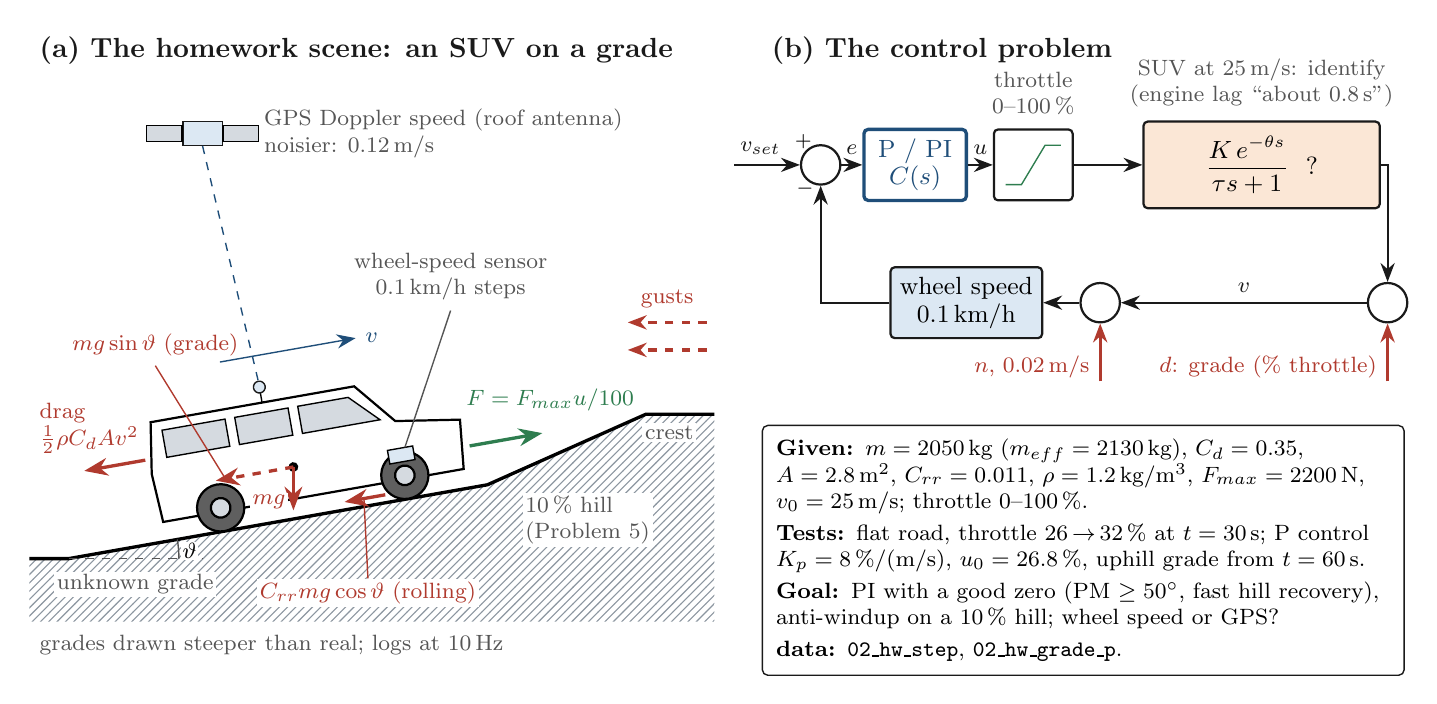
\begin{tikzpicture}
% ================= (a) the scene =================
\node[panel title] at (0,7.75) {(a) The homework scene: an SUV on a grade};
% road profile (angles exaggerated): flat, 3 % grade, 9 % hill, crest
\def\aa{10} \def\ab{24}
\coordinate (r0) at (0,1.3);
\coordinate (r1) at (0.5,1.3);
\coordinate (r2) at ($(r1)+(\aa:5.4)$);
\coordinate (r3) at ($(r2)+(\ab:2.2)$);
\fill[ground] (0,0.5) -- (r0) -- (r1) -- (r2) -- (r3) -- (8.7,0 |- r3) -- (8.7,0.5) -- cycle;
\draw[thick line] (r0) -- (r1) -- (r2) -- (r3) -- (8.7,0 |- r3);
\draw[thin line, dashed, note] (r1) -- ++(1.7,0);
\draw[thin line, note] ($(r1)+(1.4,0)$) arc (0:\aa:1.4);
\node[font=\footnotesize, fill=white, inner sep=0.5pt, anchor=west] at ($(r1)+(4:1.42)$) {$\vartheta$};
\node[caption, anchor=north west, fill=white, inner sep=1pt] at (0.3,1.15) {unknown grade};
\node[caption, anchor=north west, align=left, fill=white, inner sep=1pt] at (6.25,2.15)
     {10\,\% hill\\(Problem 5)};
\node[caption, anchor=north, fill=white, inner sep=1pt] at ($(r3)+(0.3,-0.1)$) {crest};
\node[caption, anchor=west] at (0,0.2) {grades drawn steeper than real; logs at 10\,Hz};

% car on the 3 % section, drawn in the road frame
\begin{scope}[shift={($(r1)+(\aa:3.2)$)}, rotate=\aa, scale=1.25]
  \draw[thin line, ->, accent] (-0.7,1.7) -- (0.7,1.7) node[right, font=\footnotesize] {$v$};
  \draw[fill=white] (-1.55,0.2) -- (1.55,0.2) -- (1.6,0.7) -- (0.95,0.8) -- (0.6,1.22) -- (-1.5,1.22)
        -- (-1.58,0.7) -- cycle;
  \draw[thin line, fill=metal] (-1.4,0.84) -- (-1.4,1.12) -- (-0.75,1.12) -- (-0.75,0.84) -- cycle;
  \draw[thin line, fill=metal] (-0.65,0.84) -- (-0.65,1.12) -- (-0.1,1.12) -- (-0.1,0.84) -- cycle;
  \draw[thin line, fill=metal] (0.0,0.84) -- (0.0,1.12) -- (0.52,1.12) -- (0.8,0.84) -- cycle;
  \foreach \x in {-0.95,0.95} {\draw[fill=ink!70] (\x,0.24) circle (0.24); \draw[fill=metal] (\x,0.24) circle (0.1);}
  \draw[thin line] (-0.35,1.22) -- (-0.35,1.36); \fill[sensorc, draw=ink, thin line] (-0.35,1.38) circle (0.06);
  \coordinate (gps) at (-0.35,1.44);
  \draw[fill=sensorc, thin line] (0.82,0.38) rectangle (1.08,0.52);
  \coordinate (wss) at (1.0,0.52);
  \coordinate (cg) at (-0.15,0.52);
  \fill (cg) circle (0.05);
  \draw[force, act] (1.65,0.42) -- (2.4,0.42);
  \coordinate (Ftip) at (2.4,0.42);
  \draw[force, dist] (-1.62,0.85) -- (-2.25,0.85);
  \coordinate (dragtip) at (-2.25,0.85);
  \draw[force, dist] (0.72,0.08) -- (0.3,0.08);
  \coordinate (roll) at (0.5,0.08);
  \draw[force, dist, dashed] (cg) -- ++(-0.8,0);
  \coordinate (mgs) at (-0.85,0.52);
\end{scope}
\draw[force, dist] (cg) -- ++(0,-0.55) node[left, font=\footnotesize, pos=0.8, fill=white, inner sep=0.8pt, xshift=-1.5pt] {$mg$};
% force labels
\node[font=\footnotesize, dist, anchor=south west, align=left] at (0,2.5) {drag\\$\tfrac12\rho C_d A v^2$};
\draw[thin line, dist] (roll) -- (4.3,1.05);
\node[font=\footnotesize, dist, anchor=north, fill=white, inner sep=1pt] at (4.3,1.05) {$C_{rr} m g\cos\vartheta$ (rolling)};
\draw[thin line, dist] (mgs) -- (1.6,3.75) node[above, font=\footnotesize, dist] {$m g\sin\vartheta$ (grade)};
\node[font=\footnotesize, act, anchor=south, align=center] at ($(Ftip)+(0.1,0.15)$) {$F = F_{max}u/100$};

% sensors
\draw[thin line, note] (wss) -- (5.35,4.45);
\node[caption, anchor=south, align=center] at (5.35,4.45) {wheel-speed sensor\\0.1\,km/h steps};
\node[draw=ink, thin line, fill=sensorc, minimum width=5mm, minimum height=3mm, inner sep=0pt] (sat) at (2.2,6.7) {};
\draw[thin line, fill=metal] ($(sat.west)+(-0.45,-0.1)$) rectangle ($(sat.west)+(0,0.1)$);
\draw[thin line, fill=metal] ($(sat.east)+(0,-0.1)$) rectangle ($(sat.east)+(0.45,0.1)$);
\draw[thin line, dashed, accent] (sat.south) -- (gps);
\node[caption, anchor=west, align=left] at (2.85,6.7) {GPS Doppler speed (roof antenna)\\noisier: 0.12\,m/s};
% head-wind gusts
\foreach \y in {3.95,4.3}
  \draw[distsig, dashed] (8.6,\y) -- (7.6,\y);
\node[caption, anchor=south, text=dist] at (8.1,4.35) {gusts};
% ================= (b) the control problem =================
\begin{scope}[xshift=9.3cm]
\node[panel title] at (0,7.75) {(b) The control problem};
\def\yt{6.3} \def\yb{4.55}
\node[sum] (s1) at (0.75,\yt) {};
\node[font=\scriptsize] at ($(s1)+(-0.22,0.3)$) {$+$};
\node[font=\scriptsize] at ($(s1)+(-0.2,-0.3)$) {$-$};
\draw[sig] (-0.35,\yt) -- node[above, font=\footnotesize, pos=0.4] {$v_{set}$} (s1);
\node[ctrl, minimum width=13mm] (C) at (1.95,\yt) {P / PI\\[-1pt]$C(s)$};
\node[block, minimum width=10mm] (sat) at (3.45,\yt) {};
\draw[thin line, act] ($(sat)+(-0.35,-0.25)$) -- ($(sat)+(-0.15,-0.25)$) -- ($(sat)+(0.15,0.25)$) -- ($(sat)+(0.35,0.25)$);
\node[caption, anchor=south, align=center] at ($(sat)+(0,0.5)$) {throttle\\0--100\,\%};
\node[plant, minimum width=30mm, minimum height=11mm] (eng) at (6.35,\yt) {$\dfrac{K\,e^{-\theta s}}{\tau s+1}$\ \ ?};
\node[caption, anchor=south, align=center] at ($(eng)+(0,0.6)$) {SUV at 25\,m/s: identify\\(engine lag ``about 0.8\,s'')};
\draw[sig] (s1) -- node[above, font=\footnotesize] {$e$} (C);
\draw[sig] (C) -- node[above, font=\footnotesize] {$u$} (sat);
\draw[sig] (sat) -- (eng);
% bottom row (signals flow right to left)
\node[sum] (s2) at (7.95,\yb) {};
\node[sum] (s3) at (4.3,\yb) {};
\node[sensor, minimum width=17mm] (wsens) at (2.6,\yb) {wheel speed\\[-1pt]0.1\,km/h};
\draw[sig] (eng.east) -| (s2);
\draw[sig] (s2) -- node[above, font=\footnotesize] {$v$} (s3);
\draw[sig] (s3) -- (wsens);
\draw[sig] (wsens) -- (0.75,\yb) -- (s1);
\draw[distsig] (7.95,3.55) -- node[left, font=\footnotesize, dist, pos=0.25] {$d$: grade (\% throttle)} (s2);
\draw[distsig] (4.3,3.55) -- node[left, font=\footnotesize, dist, pos=0.25] {$n$, 0.02\,m/s} (s3);

% goal box
\node[draw=ink, thin line, rounded corners=2pt, fill=white, anchor=north west, align=left,
      text width=78mm, font=\footnotesize, inner sep=5pt] at (0,3.0) {\raggedright%
  \textbf{Given:} $m = 2050$\,kg ($m_{eff} = 2130$\,kg), $C_d = 0.35$, $A = 2.8$\,m$^2$, $C_{rr} = 0.011$,
  $\rho = 1.2$\,kg/m$^3$, $F_{max} = 2200$\,N, $v_0 = 25$\,m/s; throttle 0--100\,\%.\\[2pt]
  \textbf{Tests:} flat road, throttle 26\,$\to$\,32\,\% at $t = 30$\,s; P control $K_p = 8$\,\%/(m/s),
  $u_0 = 26.8\,\%$, uphill grade from $t = 60$\,s.\\[2pt]
  \textbf{Goal:} PI with a good zero (PM $\ge 50^\circ$, fast hill recovery), anti-windup on a 10\,\% hill;
  wheel speed or GPS?\\[2pt]
  \textbf{data:} \texttt{02\_hw\_step}, \texttt{02\_hw\_grade\_p}.};
\end{scope}
\end{tikzpicture}
\end{document}
